\chapter{Ergebnisse}

\section{Energie Rekonstruktion mit Hilfe eines Random Forest Regressors}

Um ein Vergleichsergebnis zu erhalten, wird zunächst ein RandomForest Regressor, wie er in \autoref{sec:RF} beschrieben ist, verwendet,
der eine Energieschätzung für jedes Teleskop vornimmt.
Für das Training werden nur Gamma Ereignisse verwendet und somit eine erfolgreiche Signal-Untergrund Trennung vorrausgesetzt.
Es werden jedoch zerstreute und punktgerichtete Gamma Simulationsdaten verwendet, womit das Testen realitätstreuer ist, da in der
Realität die Signal Extraktion nicht zwischen punktgerichteten Photonen und Photonen, die in der Atmosphäre entstehen oder zu der
allgemeinen kosmische Strahlung gehören, unterscheiden kann.

Als Attribute werden die nicht richtungsabhängigen Hillasparameter verwendet, dazu gehören Intensität, Länge, Weite, Schiefe und Weite, sowie
die totale Intensität, die von allen Teleskopen, die das gleiche Ereignis gesehen haben, aufgenommen wird.
Zusätzlich werden die Anzahl der ausgelösten Teleskope, SST, MST und LST als Attribute verwendet, sowie die Identifikationsnummer des
Teleskopes, welche für das LST $1$, für das MST $2$ und für das SST $3$ ist.

Desweiteren werden die skalierte Länge und Weite verwendet, die durch
\begin{equation}
  SW = \frac{w- \langle w \rangle}{\sigma_w}
\end{equation}
und
\begin{equation}
  SL = \frac{l - \langle l \rangle}{\sigma_l}
\end{equation}
definiert sind, wobei der Mittelwert über alle Trainingsdatenwerte genommen wird. Diese Methode nennt sich Scaled Cuts Technik.\cite[104]{HESS}

Der ganze Datensatz besteht aus ??????????????? Datenpunkten, die durch die \textsc{train\_test\_split}-Funktion der \textsc{sklearn}-Bibliotheke
in einen Trainings und Testdatensatz aufgeteilt wird. Dabei wird mit $\SI{33}{\percent}$ der Daten trainiert und mit $\SI{66}{\percent}$
getestet. Die Aufteilung geschieht jedoch mithilfe der Ereignisnummer, damit bei der Trennung keine Ereignisse getrennt werden.

Bei dem Training werde ein Random Forest verwendet, der eine Maximal Tiefe von $10$ Ebenen besitzt, damit es nicht zum Übertraining
kommt, da der Trainingsdatensatz nur ?????????? Datenpunkte besitzt.
Jeder Baum trainiert mit $\sqrt{N}$ Attributen,wobei $N$ Attribute zur Verfügung stehen, da sonst die Bäume nicht mehr unkorreliert
sind und somit die Ergebnisse der einzelnen Bäume nicht mehr verschieden sind.
Außerdem besteht der Wald aus $100$ Bäumen, wobei dieser Parameter mit einer größeren Rechenleistung vergrößert werden kann, ohne
das es zum Übertraining kommt, was in \autoref{sec:RF} genauer erklärt ist.
Die anderen Hyperparameter sind nicht manuell verändert und somit nutzt der Algorithmus das in \autoref{sec:RF} beschriebene Kriterium der
Varianz Reduktion.
Da die gering gewählte Tiefe ein Übertraining bereits verhindern sollte und das Problem viel Statistik besitzt, werden die Hyperparameter
der minimalen Blatt und Trenngröße auf ihrer Grundeinstellung von $1$ und $2$ gelassen.

\begin{figure}
  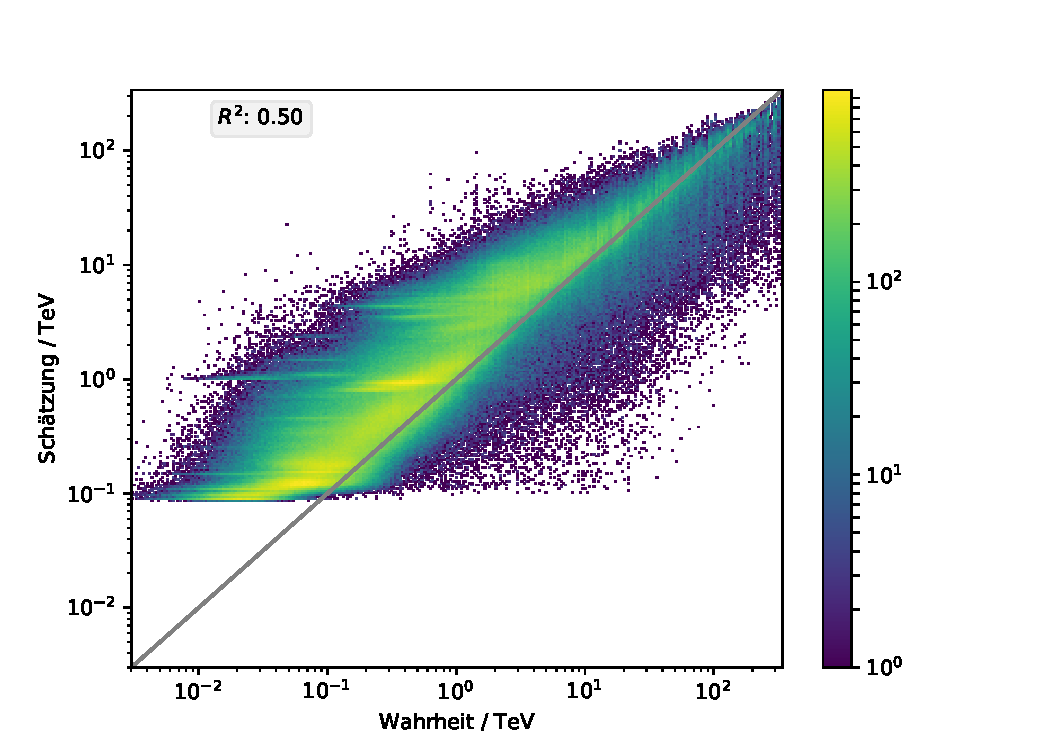
\includegraphics{Plots/RF.pdf}
  \caption{In diesem Graph ist die vorhergesagte Energie gegen die Wahrheit aufgetragen, dabei ist eine Streuung mit einer Verzerrung um die
          Diagonale zu erkennen.}
  \label{abb:Energie_RF}
\end{figure}

Dieser Entscheidungswald liefert eine Performance, wie sie in \autoref{abb:Energie_RF} zu sehen ist.
Dabei ist eine deutliche Überschätzung der Wahrheiten zu beobachten. Außerdem sind feine horizontale Linien zu sehen, die auf eine Korreliertheit
der Entscheidungsbäume hindeutet.
Der $R^2$-Wert von $\num{0.51}$ deutet jedoch daraufhin, dass der Random Forest eine bessere Beschreibung des Modells liefert als der Mittelwert.
Die Korreliertheit und die Verzerrung kann durch eine geeignetere Wahl der Hyperparameter minimiert werden, jedoch ist dies nicht das Ziel dieser
Arbeit.

\begin{figure}
  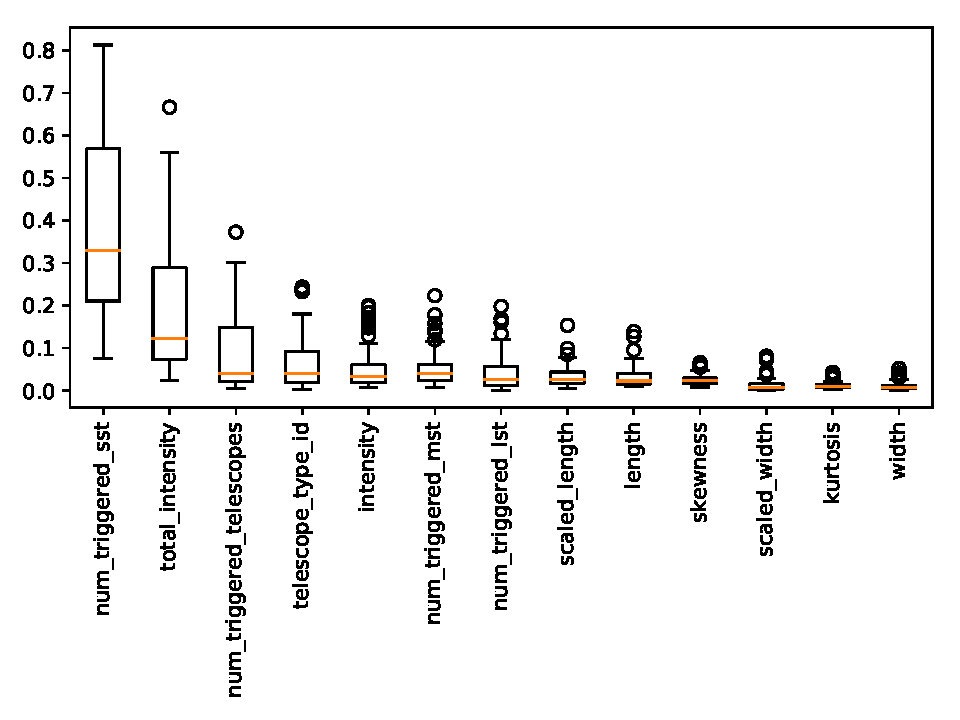
\includegraphics{Plots/feautureimportance_boxplot_trafo_firstForest.pdf}
  \caption{Darstellung der Wichtigkeit der genutzen Attribute bei der ersten Vorhersage als Boxplot.}
  \label{abb:first_FI}
\end{figure}

In \autoref{abb:first_FI} ist die Wichtigkeit der Attribute dargestellt.
% Analyse des Boxplots

\section{Optimierung durch Mittelwerte und geeignete Gewichte}

%Einfacher Mittelwert über gleiches Event; Nutzung von unterschiedlichen Gewichten;

\section{Verschachtelung von Regressionsverfahren}

%Einmal Verschachteln ; Mehrmals Verschafteln gegen die Laufzeit
